\documentclass{article}

\usepackage{cite}
\usepackage{amsmath,amssymb,amsfonts}
\usepackage{algorithmic}
\usepackage{graphicx}
\usepackage{textcomp}
\usepackage{xcolor}
\usepackage{url}
\usepackage[
    left=3cm,
    right=3cm,
    top=2cm,
    bottom=2cm
]{geometry}

\setlength{\parskip}{0.4em}

\begin{document}
\title{ATAI Evaluation Event II\\[0.3em]
\large \textit{CoralLeapingBird}}

\author{
Georgios Stratidis (\textit{h50})
\and
Diego Gobbetti (\textit{h35})
}

\date{}

\maketitle
\noindent
\textbf{Max. 2 pages.} Additional pages will not be read.
References and screenshots are excluded from the page limit.

\section{Agent Overview and Capabilities}

Our agent answers single-hop factual questions about movies from the provided knowledge graph, which is derived from Wikidata~\cite{vrandecic2014wikidata}. Every natural-language question is turned into a SPARQL query~\cite{harris2013sparql}, and the answer is read from the graph and returned as a template sentence, e.g.\ ``\textit{The factual answer is: Jeong Seo-kyeong and Park Chan-wook}''. Several answers are joined with ``and''. The agent handles both directions of a triple: the property of a movie (``\textit{Who directed Alien?}'') and the movies of a person (``\textit{Which movies did Sofia Coppola direct?}''). It also answers counts (``\textit{How many movies has Céline Sciamma directed?}''), the earliest or latest film of a person, yes/no questions (``\textit{Did Ridley Scott direct Jaws?}'' $\rightarrow$ ``No''), and single negations (``\textit{Which movies did John Ford not direct?}'', ``\textit{Which directors did not direct Jaws or Alien?}''). Titles may be quoted or unquoted, in lower case, without their article, or contain typos. When the agent cannot find the entity, the property, or the fact, it says so instead of guessing. Raw SPARQL queries from Evaluation I are still executed directly. The agent serves several chatrooms in parallel and keeps running when single requests fail.

\section{Adopted Methods}

\begin{itemize}
    \item \textbf{Knowledge graph store.} We load \texttt{graph.nt} (2.4M triples) once into an on-disk store of pyoxigraph\footnote{\url{https://pyoxigraph.readthedocs.io/}}, a SPARQL~1.1 engine written in Rust. It is built once (11\,s) and then opens in 0.01\,s; queries run outside Python's global interpreter lock, so chatrooms are answered in parallel.
    \item \textbf{Normalisation layer.} Before parsing, a rule-based preprocessor repairs quote shapes, rewrites paraphrases (``\textit{was at the helm of}'' $\rightarrow$ ``\textit{directed}''), strips trailing clauses, and resolves every title mention. It detects negation (\textit{not}, \textit{never}, \textit{n't}) only outside title mentions, so \textit{No Country for Old Men} or \textit{Never Let Me Go} are not negations. It also reads the answer class (``\textit{actors}'', ``\textit{directors}''), detects yes/no claims, and asks for clarification when a mention is unknown, e.g.\ \textit{Don't Look Up}, which contains the known film \textit{Up}.
    \item \textbf{Entity linking.} As in tutorial 04a, we build label dictionaries at startup (\texttt{ent2lbl}, \texttt{lbl2ent}; 123k labels, 5\,s). A quoted title is looked up directly; otherwise we search for the longest word sequence that is a label, with and without a leading article. For typos we fall back to fuzzy matching with RapidFuzz\footnote{\url{https://github.com/rapidfuzz/RapidFuzz}} using the optimal string alignment distance~\cite{damerau1964technique} (similarity $\geq 0.85$, $\geq 0.80$ for short titles), which counts a swap or substitution (``Godfahter'') as a single edit. Candidates with the same label are ranked films first, then by their number of triples.
    \item \textbf{Relation linking.} The question is matched against the graph's own property labels (497, e.g.\ ``director'', ``box office'') plus a small data file of everyday wordings for 26 common properties (``directed'', ``starred'', ``came out'').
    \item \textbf{Query construction.} Five SPARQL templates: lookup, count, earliest/latest film by release date, an \texttt{ASK} query for yes/no claims, and a complement query for negations, which takes the domain of the relation and removes the linked values with \texttt{FILTER NOT EXISTS}.
    \item \textbf{Platform.} Speakeasy's Python client (speakeasypy) and Python's thread pools for concurrency.
\end{itemize}

\section{Pipeline}

Figure~\ref{fig:pipeline} shows the pipeline for the question ``\textit{Which directors did not direct Jaws or Alien?}''. The message is not a SPARQL query, so it goes to the preprocessor. It resolves the mentions \textit{Jaws} (\texttt{wd:Q189505}) and \textit{Alien} (\texttt{wd:Q103569}), finds the negation ``not'' outside the titles, and reads ``directors'' as the answer class; the noun is removed so that it cannot be mistaken for the relation. The parser links ``direct'' to \texttt{wdt:P57}, and two \texttt{ASK} queries show that the answer is the object of the triple. Because the question is negated, the agent builds the complement over all directors, excluding the directors of both films (an ``or'' is read as ``neither''):
\begin{center}
\texttt{SELECT DISTINCT ?x ?label WHERE \{ ?f wdt:P57 ?x .}\\
\texttt{FILTER NOT EXISTS \{ wd:Q189505 wdt:P57 ?x \}}\\
\texttt{FILTER NOT EXISTS \{ wd:Q103569 wdt:P57 ?x \}}\\
\texttt{OPTIONAL \{ ?x rdfs:label ?label \} \}}
\end{center}
The answer starts ``\textit{The factual answer is: A.\,D.\ Miles and A.\ Edward Sutherland and \dots}'' and contains neither Steven Spielberg nor Ridley Scott. With ``\textit{Which actors \dots}'' the universe becomes the cast members (\texttt{wdt:P161}), while the relation stays \texttt{wdt:P57}.

\textbf{Limitations.}
\begin{itemize}
    \item \textbf{Complex negation.} Negation is a yes/no signal: the agent does not count negation words or work out their scope. ``\textit{Did Steven Spielberg not not direct Jaws?}'' is read as a single negation and answered with every director except Spielberg, instead of ``Yes''. A negation also switches off the yes/no path, so negated claims are answered with a list. ``\textit{neither \dots\ nor}'' is not recognised (``\textit{Who directed neither Jaws nor Alien?}'' returns Steven Spielberg), and negated counts ignore the negation (``\textit{How many movies did Steven Spielberg not direct?}'' returns 32, the number he did direct).
    \item \textbf{Size of negated answers.} The complement of one director contains almost every film in the graph; for Steven Spielberg the answer has about 200,000 characters. The bot cuts replies at 4,000 characters, but Speakeasy still rejects such messages (HTTP 400), so the user receives no reply. The first complement query after a start also exceeded the 20\,s query timeout on Nuvolos, while repeated queries take about 1.3\,s. A short reply with the number of results and a few examples would solve both problems.
    \item \textbf{Other.} A quoted unknown title is still linked to a word inside it: ``\textit{Who directed 'Don't Look Up'?}'' replies that there is no information about the director of \textit{Don}; the unquoted question is correctly refused. Questions with a literal value, such as ``\textit{Which movies came out in 1984?}'', are out of scope: the agent links the film \textit{1984} and returns its release date.
\end{itemize}

\section{Improvements}

\textbf{Faster and parallel graph access.} Our first agent parsed the 290\,MB graph with rdflib at every start and answered one message at a time. The persistent store and a worker pool with one lock per chatroom answer rooms in parallel while keeping the order within a room; the median answer time of non-negated questions is below 10\,ms.

\textbf{Adversarial question forms.} Our first submission ignored negation and answered ``\textit{Who did not direct Notting Hill?}'' with Roger Michell, its director. It also answered for a known fragment of an unknown title: ``\textit{who directed don't look up}'' returned the directors of \textit{Up}. We built ten test sets of adversarial forms (negation, titles inside titles, quote shapes, typos, partial titles, counts, several mentions, trailing superlatives, yes/no questions, paraphrases), checked against hand-written SPARQL. The first agent passed 172 of 607 cases; with the normalisation layer it passes all 664 cases, including 57 more negation cases with director and actor answer classes, several films, and people without directing credits (``\textit{What did Marilyn Monroe not direct?}'').

\textbf{No regressions.} The regression set grew from 57 to 508 questions and still passes completely, as do the 9 SPARQL queries from Evaluation I.

\section{Additional Features}

\begin{itemize}
    \item \textbf{SPARQL pass-through} (Evaluation I): queries with or without \texttt{PREFIX} lines, also wrapped in \texttt{'''} or code fences, are executed directly.
    \item \textbf{Robustness:} timeouts for queries (20\,s) and replies (25\,s), fallback replies on errors, two attempts per posted message, automatic re-login with exponential back-off, and a heartbeat in the log.
    \item \textbf{Testing:} an offline command-line interface that prints each pipeline step (preprocessor plan, parsed question, SPARQL query), 138 unit tests on small fixture graphs, the 508-question regression set, and the 664 adversarial cases; all pass.
\end{itemize}

\begin{figure}[p]
    \centering
    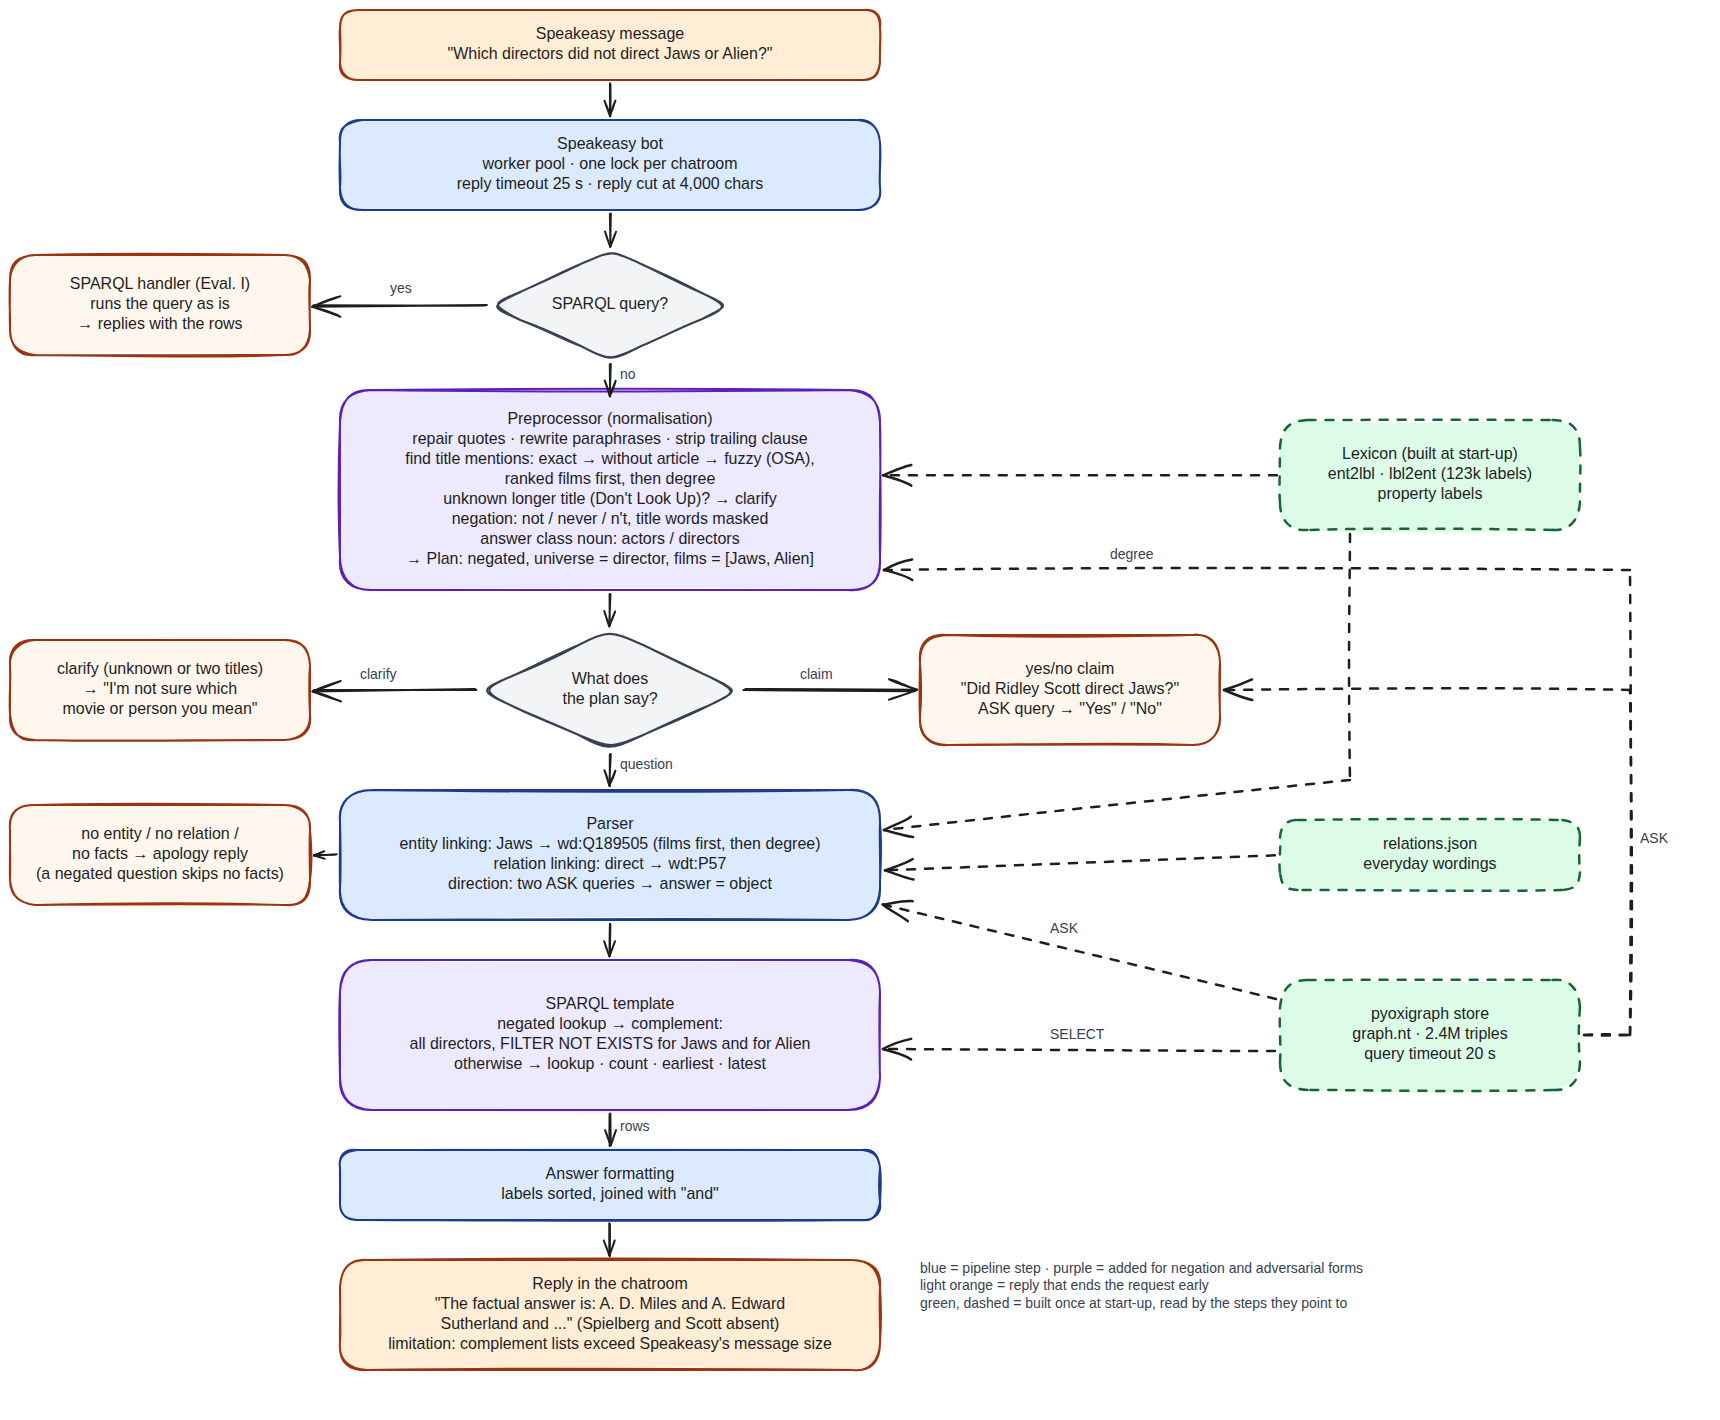
\includegraphics[width=\textwidth]{pipeline.png}
    \caption{Pipeline of the agent for a negated question. Purple steps were added for negation and other adversarial question forms; light orange boxes end the request early with their own reply; green, dashed boxes are built once at start-up.}
    \label{fig:pipeline}
\end{figure}

\bibliographystyle{abbrv}
\bibliography{references}

\end{document}
